\documentclass[11pt,a4paper]{article}

\usepackage[a4paper, margin=2.5cm]{geometry}
\usepackage{subcaption}
\usepackage[T2A]{fontenc}
\usepackage[utf8]{inputenc}
\usepackage[russian]{babel}
\usepackage{xcolor}
\usepackage{amsmath,amssymb,amsfonts}
\usepackage{graphicx}
\usepackage{indentfirst}
\usepackage{booktabs}

\usepackage{hyperref}

\title{\textbf{Адаптивный выбор параметров распределения сэмплирования 
для Monte Carlo оценки сходимости оптимизационной поверхности}}

\author{Еникеев Арнольд и Никита Киселёв}
\date{}

\begin{document}

\maketitle

\begin{abstract}
Исследование поведения функции потерь возле минимума является важной задачей для работы нейросетей и для поиска оптимального размера обучающей выборки.
\newline
Распределенный подход к оценке сходимости поверхности функции потерь использует Monte Carlo сэмплирование из гауссовского распределения в окрестности минимума.
\newline
Предыдущие исследования показали, что оценка сильно зависит от дисперсии сэмплирования.
Целью исследования является разработка адаптивных методов выбора параметров распределения сэмплирования на основе свойств кривизны оптимизационной поверхности и проведение сравнительного анализализа различных стратегий выбора.
\newline
В данной работе предлагается метод, использующий свойства матрицы Гессе для более точной оценки сходимости поверхности функции потерь.
Различные стратегии выбора сравниваются на задаче классификации изображений.
\newline
Развитие исследований в этом направлении сделает распределенный подход более практичным и устойчивым.
\newline
Результаты будут полезны для анализа локальных свойств ландшафта функции потерь и для исследования задачи определения оптимальной обучающей выборки.
\end{abstract}

\section{Введение}
% \cite{vapnik1995nature}
% \cite{bishop2006pattern} \cite{kaplan2020scaling}
%\cite{hoffmann2022training} \cite{li2018visualizing}
\begin{figure}[h]
  \centering
  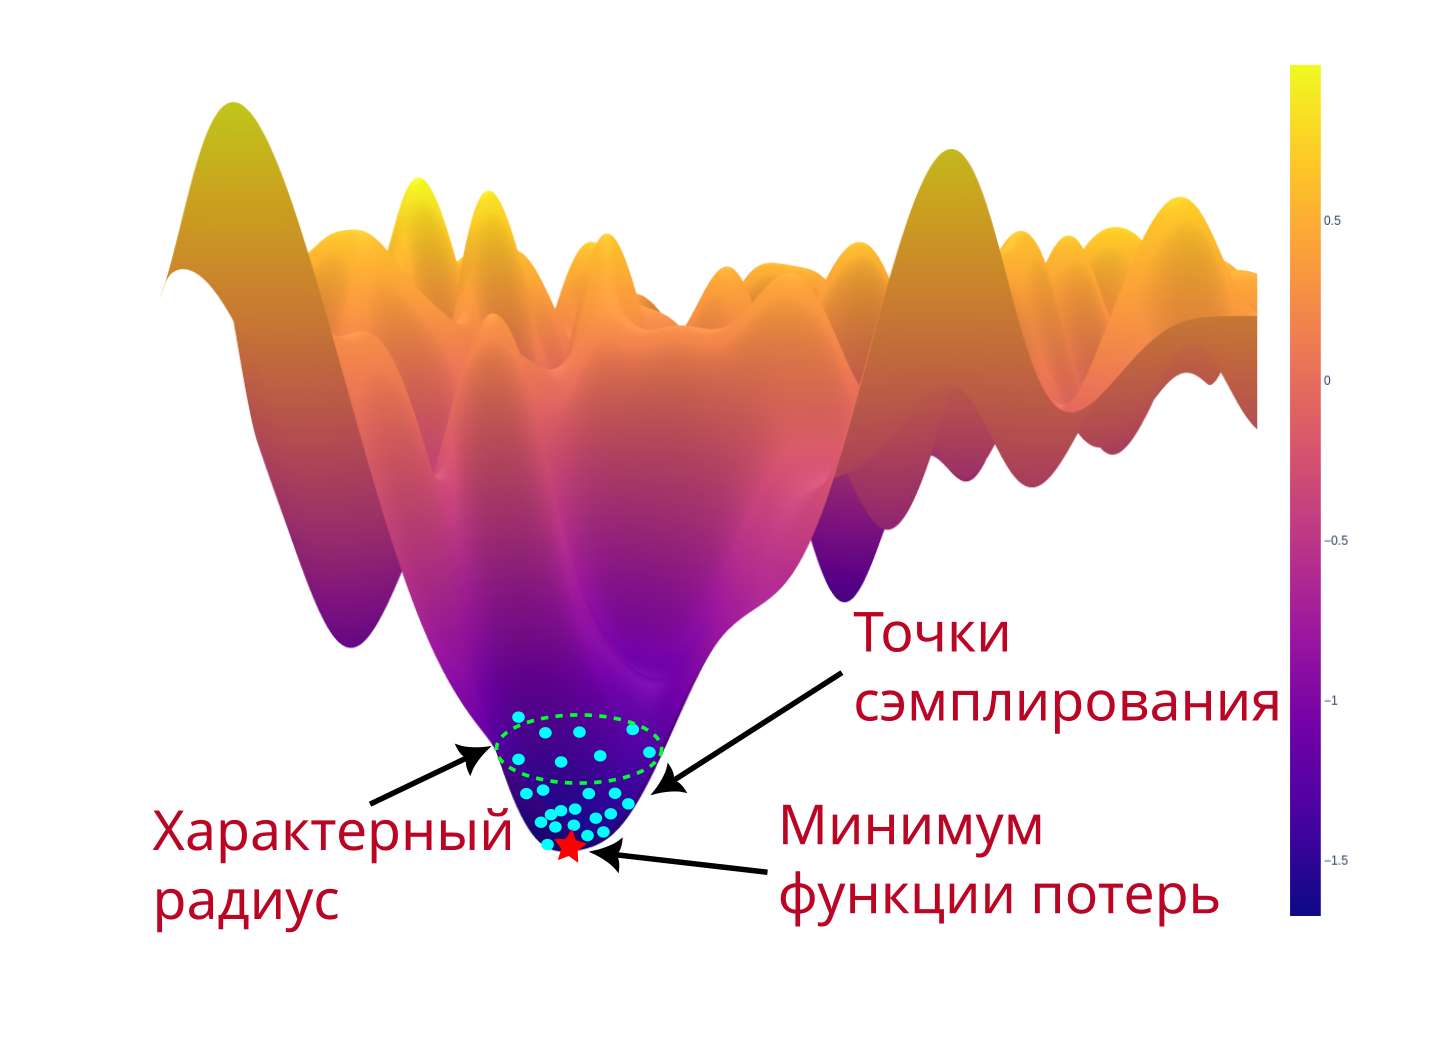
\includegraphics[width=0.6\textwidth]{pic/landscape.png}
  \caption{Критерий выбора параметра $\sigma$: точки сэмплирования должны попадать в шар характерного радиуса с центром в минимуме $\mathcal{L}(\mathbf{w}^*)$}
\end{figure}

В статистической теории машинного обучения \cite{vapnik1995nature} качество модели напрямую зависит от размера обучающей выборки. Для параметрических моделей функция потерь вычисляется по ограниченному набору данных, поэтому существует важная задача по определению оптимального размера обучающей выборки.
Для этого исследуется сходимость ландшафта функции потерь в зависимости от размера выборки \cite{kiselev2025likelihood}. Когда геометрия оптимизационной поверхности в окрестности минимума перестаёт значительно менятся при добавлении нового элемента, размер обучающей выборки считается оптимальным .


В предыдущих исследованиях \cite{kiselev2025posterior} были предложены критерии оценки сходимости оптимизационной поверхности при увеличении размера выборки, использующие гауссовское сэмплирование в окрестности минимума $\mathcal{L}(\mathbf{w})$. В \textcolor{red}{[Процитировать статью, которая ещё не вышла]} вводятся ещё два критерия: Quadratic Monte-Carlo и Gaussian-moment quadratic estimator, которые более эффективны с вычислительной точки зрения, а также доказывается их сходимость. 

Однако, для практического использования критериев Quadratic Monte-Carlo и Gaussian-moment quadratic estimator недостаточно  теоретической сходимости: необходимо, чтобы точки сэмплирования попадали в область, где ландшафт описывается квадратичной аппроксимацией Тейлора в окрестности $\mathbf{w}^{*}$ с высокой точностью \cite{meshkov2024convnets}. В таком случае данные критерии  корректно отражают сходимость оптимизационной поверхности при росте объёма выборки.

Наша задача состоит в том, чтобы найти радиус $R$ такой, что в шаре $\mathcal{B}_R(\mathbf{w}^*)$ функция потерь описывается квадратичной аппроксимацией с заданной точностью, и предложить метод выбора параметра $\sigma$, при котором гауссовское сэмплирование с заданной вероятностью попадает в данный шар \cite{kiselev2025robust}. Это позволит эффективно использовать квадратичные критерии на практике. Также необходимо будет проверить корректность предложенного метода выбора параметра $\sigma$ на практике.


\section{Связанные работы}

\textbf{Исследование зависимости ландшафта функции потерь от размера обучающей выборки.} Анализ зависимости обучения параметрической модели от размера выборки является важной задачей в классической теории обучения \cite{vapnik1995nature}. В недавних исследованиях были предложены критерии оценки сходимости ландшафта функции потерь при увиличении объёма данных \cite{kiselev2025likelihood, kiselev2025posterior, Grabovoy2022Numerical}, в частности, квадратичный критерий $\Delta_2$ и абсолютный критерий $\Delta_1$, а также показана их сходимость.
В \cite{kiselev2025robust} предложена идея делать гауссовское сэмплирование точек по Монте-Карло для оценки сходимости на практике. В статье \textcolor{red}{[Процитировать статью, которая ещё не вышла]} предложены критерии Quadratic Monte-Carlo и Gaussian-moment quadratic estimator, которые более эффективны с вычислительной точки зрения, однако их практическая применимость требует гарантии корректности аппроксимации Тейлора 2 порядка с заданной точностью . 

В нашей работе мы предлагаем адаптивный метод выбора параметра $\sigma$ на основе структуры матрицы Гессе функции потерь в минимуме \cite{kiselev2024hessian}, при котором гарантируется выполнение квадратичной аппроксимации с заданной точностью. 
В отличие от предыдущих работ, мы получаем точное выражение для параметра $\sigma$ и показываем его корректность на численном эксперименте, а не работаем в абстрактной области корректности аппроксимации Тейлора 2 порядка.


\textbf{Ландшафт функции потерь и его локальная геометрия}. 
Изучению локальной геометрии функции потерь посвящено значительное количество работ, предлагающих теоретический анализ и различные подходы к визуализации ландшафта \cite{li2018visualizing, xu2024visualizing, FortGanguli2019Emergent}. В частности, в них были описаны особенности кривизны ландшафта и спектральные свойства матрицы Гессе\cite{sagun2017empirical, ghorbani2019investigation, wu2021dissecting}.
\newline
Предыдущие исследования показали, что на практике ландшафт функции потерь крайне анизотропен, то есть значительная часть спектра матрицы Гессе имеет околонулевые значения \cite{baskerville2021appearance, singh2023hessian, Papyan2020Traces}. В недавних исследованиях для практического изучения ландшафта функции потерь была предложена идея сэмплирования в подпространстве наибольшей кривизны, то есть подпространство $d$ главных собственных векторов матрицы Гессе $\mathbf{H}$ \cite{kiselev2025robust}. В нашей работе мы развиваем данную идею и предлагаем метод выбора параметра $\sigma$ для сэмплирования в данном подпространстве и показываем, что при таком выборе $\sigma$ сэмплирование будет отражать локальные свойства минимума $\mathcal{L}(\mathbf{w})$.

\textbf{Локальные свойства ландшафта в методах оптимизации.}
Также ряд работ был посвящён изучению связи геометрии ландшафта функции потерь и структуры матрицы Гессе с работой методов стохастической оптимизации \cite{Papyan2019FullSpectrum, Dexter2024SGDStability}. 
Для функции потерь параметрических моделей разделяют flat (плоские) и sharp (острые) минимумы по кривизне поверхности в их окрестности\cite{hochreiter1997flat}.
В частности, согласно результатам исследований, в случае flat минимумов параметрическая модель обладает большей обобщающей способностью \cite{dinh2017sharp, foret2021sharpness, keskar2017largebatch}. \newline
Было показано, что стохастические методы, такие как SGD, за счёт недетерминированных обновлений обычно приводят к решениям в более плоских минимумах \cite{WuWangSu2022Alignment}. В недавних работах было изучено, как ведут себя траектории SGD на всём пространстве параметров и в подпространствах наибольшей кривизны \cite{zhou2025bsfa, song2025sgdsubspace}. В методах оптимизации важно понимать, как устроена окрестность минимума и уметь исследовать структуру ландшафта в подпространствах собственных векторов матрицы Гессе, что тесно пересекается с нашей работой \cite{Azadbakht2022KernelSharing, kiselev2024hessian}.
В отличие от других исследований, в нашей работе мы также предлагаем численные оценки для характерного радиуса корректности аппроксимации Тейлора 2 порядка и показываем, как использовать полученное выражение для исследования свойств минимума с помощью гауссовского сэмплирования. Результаты будут полезны для изучения sharp и flat минимумов и в анализе связи работы SGD со структурой матрицы Гессе.

\section{Постановка задачи}
Пусть $\mathcal{L}_k(\mathbf{w})$ -- функция потерь модели с параметрами $\mathbf{w} \in \mathbb{R}^N$ на выборке размера $k$. \newline
\text{Минимум функции потерь $\mathbf{w}_k^*:$}
$$\mathbf{w}_k^* = \arg\min_{\mathbf{w} \in \mathbb{R}^N} \mathcal{L}_k(\mathbf{w})$$
В предположении, что $\mathcal{L}_k(\mathbf{w})$ дважды непрерывно дифференциируема, верна аппроксимация Тейлора второго порядка
$$\mathcal{L}_k(\mathbf{w}) = \mathcal{L}_k(\mathbf{w}_k^*)+
\nabla\mathcal{L}_k(\mathbf{w}_k^*)^T(\mathbf{w}-\mathbf{w}_k^*)+
\frac{1}{2}(\mathbf{w}-\mathbf{w}_k^*)^T\mathbf{H_k}(\mathbf{w}-\mathbf{w}_k^*)+
o(|\mathbf{w} - \mathbf{w}_k^*|^2)$$
$\mathbf{H}_k = \nabla^2 \mathcal{L}_k(\mathbf{w}_k^*)$ -- матрица Гессе функции потерь в точке минимума.\newline
Для исследования ландшафта оптимизационной поверхности используется Monte-Carlo сэмплирование в окрестности минимума $\mathbf{w}_k^{*}$.\newline
Предлагается делать сэмплирование в подпространстве наибольшей кривизны, то есть подпространстве, образованном $d$ собственными векторами матрицы Гессе, отвечающим её $d$ наибольшим собственным значениям. Обозначим через
$$\mathbf{U}_d = [\mathbf{u}_1, \dots, \mathbf{u}_d] \in \mathbb{R}^{N \times d}$$
матрицу, составленную из этих собственных векторов. \newline
Тогда точки сэмплирования будут выглядеть следующим образом:

$$\mathbf{w} = \mathbf{w}_k^{*} + \mathbf{U}_d \mathbf{z}$$ 
$$\mathbf{z} \sim \mathcal{N}(\mathbf{0}, \sigma^2 \mathbf{I}_d)$$
где $\mathbf{I}_d$ --- единичная матрица размерности $d$. \newline
Итак, цель работы - найти такое значение параметра $\sigma^*$, при котором сэмплирование
$$\mathbf{w} = \mathbf{w}^{*} + \mathbf{U}_d \mathbf{z}$$ 
$$\mathbf{z} \sim \mathcal{N}(\mathbf{0}, \sigma^2 \mathbf{I}_d)$$
будет наиболее точно отражать локальные свойства оптимизационной поверхности в окрестности минимума и обеспечивать корректность квадратичной аппроксимации, необходимой для применения критериев Quadratic Monte-Carlo и Gaussian-moment quadratic estimator. \newline
Если говорить строго, то мы хотим найти параметр $\sigma^*_k$, для которого выполнено:
$$\sigma^*_k = \sup (\sigma > 0 :\mathbb{P}\!\left(\|\mathbf{w}-\mathbf{w}_k^*\| < R_k\right) > 1-\varepsilon),$$
где $R_k$ -- характерный радиус шара с центром в $\mathbf{w}_k^*$, для которого корректна аппроксимация Тейлора второго порядка, а $\varepsilon$ -- требуемая точность. \newline
Теоретическая значимость работы состоит в том, что предложенный метод выбора параметров позволит на практике использовать сильные квадратичные критерии для оценки сходимости ландшафта функции потерь при увеличении размера выборки. Результаты также будут полезны в анализе структуры оптимизационной поверхности.


\section{Метод выбора параметра $\sigma$}
Для определения значения $\sigma^*$ будем использовать переход к подпространству наибольшей кривизны. Обозначим за $\mathbf{U}_d = [\mathbf{u}_1, \dots\mathbf{u}_d]$ матрицу из $d$ главных собственных векторов матрицы $\mathbf{H}$. Тогда подпространство наибольшей кривизны это $\mathcal{L}in([\mathbf{u}_1, \dots\mathbf{u}_d])$ и в нём матрица Гессе будет равна $\mathbf{H}_d = \mathbf{U}_d^T\mathbf{H}\mathbf{U}_d = diag(\lambda_1, \dots \lambda_d)$, где $\lambda_1, \dots \lambda_d$ - $d$ наибольших собственных значений $\mathbf{H}$. \newline
Точки сэмплирования будут иметь следующий вид:
$$\mathbf{w} = \mathbf{w}^{*} + \mathbf{U}_d \mathbf{z}$$ 
$$\mathbf{z} \sim \mathcal{N}(\mathbf{0}, \sigma^2 \mathbf{I}_d)$$
В таком случае, получаем, что у $\mathbf{H}_d$ будут большие положительные собственные значения, что пригодится в дальнейшей оценке параметра $\sigma^*$.
\section{Теоретический анализ}
Здесь и далее считаем, что $N$ и $k$ из постановки зафиксированы, поэтому опустим индексы в обозначении функции потерь и минимума, а также используется 2-норма. \newline
%Предположение: в окрестности минимума матрица Гессе - липшицева. То есть существует $r > 0$ такой, что для любого $\mathbf{w} \in$ $\mathcal{B}_r(\mathbf{w}^*)$ выполнено $$||\mathbf{H}(\mathbf{w})-\mathbf{H}(\mathbf{w}^*)||_2 \leq C$$
В окрестности минимума $\nabla\mathcal{L}(\mathbf{w}^*) = 0$, а значит, аппроксимация Тейлора второго порядка принимает следующий вид:
$$\mathcal{L}(\mathbf{w}^* + \mathbf{h}) = \mathcal{L}(\mathbf{w}^*)+\frac{1}{2}\mathbf{h}^T\mathbf{H}\mathbf{h}+\rho(\mathbf{h})$$
Где $\mathbf{h} = \mathbf{w} - \mathbf{w}^*$, $\mathbf{h}\in \mathbb{R}^N$, а $\rho$ - остаточный член. \newline
Мы хотим, чтобы аппроксимация Тейлора второго порядка была корректна в окрестности минимума, то есть остаточный член должен быть мал по сравнению с квадратичной частью. \newline

\textbf{Лемма 1}: В подпространстве наибольшей кривизны для радиуса $R_{\psi} = \frac{3\psi \lambda_{min}(\mathbf{H_d})}{L_{\mathbf{H}}}$ для точек из шара $\mathcal{B}_{R_{\psi}}(\mathbf{w}^*)$ в 2-норме остаточный член аппроксимации Тейлора второго порядка удовлетворяет неравенству $$|\rho(\mathbf{h})| \leq \psi \times\frac{1}{2}|\mathbf{h}^T\mathbf{H}_d\mathbf{h}|$$\newline
Где $\mathbf{H}_d$ - матрица Гессе в подпространстве наибольшей кривизны, $\lambda_{min}(\mathbf{H}_d)$ - её минимальное собственное значение, а $L_{\mathbf{H}}$ - константа Липшица для $\mathbf{H}$. \newline
То есть квадратичная часть описывает поведение функции в окрестности минимума с точностью $\psi$. \newline
\textbf{Доказательство}: \newline
Из аппроксимации Тейлора второго порядка с остаточным членом в интегральной форме известно:
$$\displaystyle \rho(\mathbf{h}) =  \int_0^1 (1-t)\mathbf{h}^T ( \nabla^2\mathcal{L}(\mathbf{w}^* + t \mathbf{h})-\nabla^2\mathcal{L}(\mathbf{w}^*))\mathbf{h}dt $$
Предположение: матрице Гессе - липшицева с константой Липшица $L_{\mathbf{H}}$:
$$\|\nabla^2 \mathcal{L}(\mathbf{u}) - \nabla^2 \mathcal{L}(\mathbf{v})\|_2 \le L_\mathbf{H} \|\mathbf{u} - \mathbf{v}\|_2 \quad \forall\, \mathbf{u}, \mathbf{v} \in \mathcal{B}_r(\mathbf{w}^*)$$
Оценим остаточный член $\rho(\mathbf{H})$:
$$\displaystyle |\rho(\mathbf{h})| =  \left|\int_0^1 (1-t)\mathbf{h}^T ( \nabla^2\mathcal{L}(\mathbf{w}^* + t \mathbf{h})-\nabla^2\mathcal{L}(\mathbf{w}^*))\mathbf{h}dt \right| \leq$$ $$\leq \int_0^1 ||\mathbf{h}||^2(1-t) || \nabla^2\mathcal{L}(\mathbf{w}^* + t \mathbf{h})-\nabla^2\mathcal{L}(\mathbf{w}^*)||dt$$
Используем липшицевость:
$$ \int_0^1 ||\mathbf{h}||^2(1-t) || \nabla^2\mathcal{L}(\mathbf{w}^* + t \mathbf{h})-\nabla^2\mathcal{L}(\mathbf{w}^*)|| \leq \int_0^1 ||\mathbf{h}||^2(1-t)L_{\mathbf{H}} ||t\mathbf{h}||dt=$$ $$ = \int_0^1||\mathbf{h}||^3L_{\mathbf{H}}t(1-t)dt=\frac{1}{6}L_{\mathbf{H}}||\mathbf{h}||^3$$
Итоговая оценка на $\rho(\mathbf{h})$:
$$|\rho(\mathbf{h})| \leq \frac{1}{6}L_{\mathbf{H}}||\mathbf{h}||^3$$ \newline
Аппроксимация Тейлора 2 порядка будет хорошо приближать функцию в случае, если квадратичный член будет описывать разность $\mathcal{L}(\mathbf{w}^* + \mathbf{h}) - \mathcal{L}(\mathbf{w}^*)$, то есть если $\rho(\mathbf{h})$ будет мало относительно $\frac{1}{2}\mathbf{h}^T\mathbf{H}\mathbf{h}$, или же $$|\rho(\mathbf{h})| \leq \psi \times\frac{1}{2}|\mathbf{h}^T\mathbf{H}\mathbf{h}|$$ для $\psi > 0$, который отражает насколько точную мы хотим аппрокимацию. \newline
Получаем
$$|\rho(\mathbf{h})| = \frac{1}{6}L_{\mathbf{H}}||\mathbf{h}||^3 \leq \frac{\psi}{2} |\mathbf{h}^T\mathbf{H}\mathbf{h}|$$
При переходе к сэмплированию в подпространстве $d$ главных собственных векторов у матрицы Гессе останутся только большие собственные значения.
\newline
Далее будем считать, что мы работаем в подпростанстве главных собственных векторов. \newline
Матрицу Гессе в новом пространстве будем обозначать $\mathbf{H}_d:= \mathbf{U^{\text{T}}HU}$, где $\mathbf{U}$ - матрица перехода к подпространству главных собственных векторов. \newline
Тогда в этом подпространстве оценка на $\rho(\mathbf{h})$ будет выглядеть следующим образом:
$$|\rho(\mathbf{h})| = \frac{1}{6}L_{\mathbf{H}_d}||\mathbf{h}||^3 \leq \frac{\psi}{2} |\mathbf{h}^T\mathbf{H}_d\mathbf{h}|$$
Пусть минимальное собственное значение матрицы Гессе - $\lambda_{min}(\mathbf{H}_d)$. \newline
Сэмплирование имеет одинаковую дисперсию по каждой компоненте, поэтому, чтобы оставаться в рамках квадратичной аппроксимации, неравенство на $\rho(\mathbf{h})$ должно выполняться для всех возможных направлений $\mathbf{h}$ в подпространстве главных собственных векторов, в том числе для $\displaystyle \inf_{||\mathbf{u}|| =||\mathbf{h}||}\frac{1}{2}\mathbf{u}^T\mathbf{H}_d\mathbf{u}$, где $\mathbf{u}\in \mathbb{R}^d$. 
\newline
Оценим выражение $\frac{1}{2}\mathbf{u}^T\mathbf{H}_d\mathbf{u}$. \newline
Для этого разложим $\mathbf{u}$ по главным собственным векторам матрицы Гессе:
$$\displaystyle \mathbf{u} = \sum_{j=1}^d \theta_j \mathbf{e}_j$$
Где $\{ \mathbf{e}_j \}_{j=1}^d$ - собственные вектора $\mathbf{H}_d$. \newline
Тогда сделаем оценку:
$$\frac{1}{2}\mathbf{u}^T\mathbf{H}_d\mathbf{u}=\frac{1}{2}\left( \sum_{j=1}^d \theta_j \mathbf{e}_j \right)^T \mathbf{H}_d \left( \sum_{j=1}^d \theta_j \mathbf{e}_j \right) = \frac{1}{2}\left( \sum_{j=1}^d \theta_j \mathbf{e}_j \right)^T \left( \sum_{j=1}^d \theta_j \lambda_j(\mathbf{H}_d)\mathbf{e}_j \right) = $$ $$=\sum_{j=1}^d \theta_j^2 ||\mathbf{e}_j||^2\lambda_j(\mathbf{H}_d) \geq \frac{1}{2}\lambda_{min}(\mathbf{H}_d)\sum_{j=1}^d \theta_j^2 ||\mathbf{e}_j||^2 = \frac{1}{2}\lambda_{min}(\mathbf{H}_d)||\mathbf{u}||^2 = \frac{1}{2}\lambda_{min}(\mathbf{H}_d)||\mathbf{h}||^2$$
В переходах было использованно то, что базис ортонормированный, что $\mathbf{H}_d\mathbf{e}_j=\lambda_{j}\mathbf{e}_j$ и что сумма квадратов коэффициентов разложения $\theta_j$ это норма вектора $\mathbf{u}$.
То есть, если мы оценим квадратичную часть снизу через $\lambda_{min}(\mathbf{H}_d)$, то для полученных $\rho$ квадратичная аппроксимация будет тем более работать.
Следовательно, оценка для $\rho$ принимает вид:
$$\rho(\mathbf{h}) = \frac{1}{6}L_{\mathbf{H}_d}||\mathbf{h}||^3 \leq  \frac{\psi \lambda_{min}(\mathbf{H}_d)}{2}||\mathbf{h}||^2$$
Из чего получаем:
$$||\mathbf{h}|| \leq \frac{3\psi \lambda_{min}(\mathbf{H_d})}{L_{\mathbf{H}_d}}$$
Получаем, что для радиуса $R_{\psi} = \frac{3\psi \lambda_{min}(\mathbf{H_d})}{L_{\mathbf{H}_d}}$ точки из шара $\mathcal{B}_{R_{\psi}}(\mathbf{w}^*)$ в 2-норме будут соответствовать именно части ландшафта оптимизационной поверхности, в которой корректна аппроксимация Тейлора 2 порядка. \newline
\textbf{Лемма 1} доказана. \newline
Вернёмся к параметру $\sigma^*$.


\textbf{Теорема 1}: Пусть в подпространстве $d$ главных собственных векторов матрицы Гессе осуществляется сэмплирование:
$$\mathbf{w} = \mathbf{w}^{*} + \mathbf{U}_d \mathbf{z}$$ 
$$\mathbf{z} \sim \mathcal{N}(\mathbf{0}, \sigma^2 \mathbf{I}_d)$$
Характерный радиус области корректности квадратичной аппроксимации равен
$$R_{\psi} = \frac{3 \psi \lambda_{\min}(\mathbf{H}_d)}{L_{\mathbf{H}_d}}.$$
Тогда максимальное значение параметра $\sigma^{*}$, при котором гауссовское сэмплирование попадает в $\mathcal{B}_{R_\psi}(\mathbf{w}^*)$ с вероятностью не менее $1-\varepsilon$, задаётся формулой

$$\sigma^{*} =
\sqrt{\frac{9 \psi^2 \lambda_{\min}^2(\mathbf{H}_d)}{{L}_{\mathbf{H}_d}^2 \chi^2_{1-\varepsilon}(d)}}$$
\textbf{Доказательство}:\newline
Рассмотрим формулу для $\sigma^*$:\newline
$$\sigma^* = \sup (\sigma > 0 :\mathbb{P}\left(\|\mathbf{w}-\mathbf{w}^*\| < R\right) > 1-\varepsilon),$$
Подставим $R = R_{\psi}$:
$$\sigma^* = \sup (\sigma > 0 :\mathbb{P}\!\left(\|\mathbf{w}-\mathbf{w}^*\| < \frac{3\psi \lambda_{min}(\mathbf{H_d})}{L_{\mathbf{H}_d}}\right) > 1-\varepsilon),$$
Осталось подобрать дисперсию так, чтобы гауссовское сэмплирование попадало в нужный интервал с вероятностью $1-\varepsilon$. \newline
То есть нужно решить следующую задачу:\newline
Задан радиус $r > 0$. \newline
Для $d$-мерного гауссовского распределения $\mathcal{N}(\mathbf{0}, \sigma^2 \mathbf{I}_d)$ нужно максимальное $\sigma$, для которого хотя бы $(1-\varepsilon)$ая часть точек будет попадать в $\mathcal{B}_r(\mathbf{0})$ в 2-норме. \newline
Значит, мы хотим, чтобы для сэмплирования распределения $\mathcal{N}(\mathbf{0}, \sigma^2 \mathbf{I}_d)$ размера $S$ точек $\{\mathbf{\xi}_l\}^{l=S}_{l=1}\in\mathbb{R}^d$ выполнялось:
%$$\mathbb{E} ( \#l:\xi_l\in\mathcal{B}_r(0) ) > (1-\varepsilon)S$$
%Или, равносильно:
$$\mathbb{P} ( \xi\in\mathcal{B}_r(\mathbf{0}) ) > (1-\varepsilon)$$
Пусть $\xi = \sigma \eta$. \newline
Тогда $\eta \sim \mathcal{N}(\mathbf{0}, \mathbf{I}_d)$. Значит $||\eta||^2= \displaystyle \sum_{i=1}^d \eta_i^2 \sim \chi^2(d)$. \newline
Получаем:
$$\mathbb{P}\left(\xi\in\mathcal{B}_r(\mathbf{0})\right) = \mathbb{P}\left(||\xi||^2 < r^2\right) = \mathbb{P}\left(||\eta||^2 < \frac{r^2}{\sigma^2}\right) > 1 - \varepsilon$$
Обозначим $\zeta =||\eta||^2= \displaystyle \sum_{i=1}^d \eta_i^2 \implies \zeta \sim \chi^2(d).$ Следовательно:
$$\mathbb{P}\left(\xi\in\mathcal{B}_r(\mathbf{0})\right)=\mathbb{P}\left(\zeta < \frac{r^2}{\sigma^2}\right) > 1-\varepsilon$$
Значит, в граничном случае, когда достигается супремум, получается:
$$\mathbb{P}\left(\zeta < \frac{r^2}{(\sigma^*)^2}\right) = 1-\varepsilon$$
Следовательно:
$\frac{r^2}{(\sigma^*)^2} = \chi^2_{1-\varepsilon}(d)$, то есть 
$$(\sigma^*)^2=\frac{r^2}{\chi^2_{1-\varepsilon}(d)}$$
Подставим найденное в рамках задачи $R_{\psi}$, чтобы получить итоговое выражение для $\sigma^*$:
$$\sigma^* = \sqrt{\frac{9\psi^2 \lambda_{min}^2(\mathbf{H}_d)}{L_{\mathbf{H}_d}^2\chi^2_{1-\varepsilon}(d)}}$$
\textbf{Теорема 1 доказана.}
    

\textbf{Замечание 1:} На практике точное вычисление константы Липшица $L_{\mathbf{H}_d}$ для параметрических моделей проблематично, поскольку пространство параметров имеет большую размерность. Соответственно, величины $R_{\psi}$ и $\sigma^{*}$ также считаются приближённо. \newline
В вычислительных экспериментах мы используем для константы Липшица cледующую оценку: 
$L_{\mathbf{H}_d}$ оценивается через $\frac{||\mathbf{H}_d(t\mathbf{v}) - \mathbf{H}_d(\mathbf{0})||}{t}$ при малых $t > 0$, для $D$ случайных направлений $\mathbf{v}$ в подпространстве наибольшей кривизны.


\textbf{Замечание 2:}
Из полученного выражения видно, что выбор размерности подпространства $d$ существенно влияет на значение $\sigma^{*}$. При увеличении $d$ растёт и квантиль $\chi^2_{1-\varepsilon}(d)$, следовательно, уменьшается $\sigma^{*}$. В то же время уменьшается $\lambda_{min}(\mathbf{H}_d)$, что также приводит к уменьшению $\sigma^{*}$. Как было показано в предыдущих исследованиях, пространство параметров крайне анизотропно, поэтому важно уметь правильно подбирать $d$, чтобы подпространство наибольшей кривизны хорошо приближало исходное, но в то же время не брать достаточно большое $d$, при котором $\lambda_{min}(\mathbf{H}_d)$ будет мало.

\section{Вычислительный эксперимент}
Вычислительный эксперимент проводился для модели ResNet-18 на датасете CIFAR-10. После обучения модели в полученном минимуме функции потерь $\mathbf{w}^*$ вычислялись главные собственные значения и собственные вектора матрицы Гессе через power iteration с использованием Hessian-vector-product. Для фиксированного $d$ строилось подпространство наибольшей кривизны, то есть линейное пространство, построенное на $d$ главных собственных векторах $\mathbf{H}$, и матрица Гессе $\mathbf{H}_d$ в нём:
$$\mathbf{H}_d = \mathbf{U}_d^T \mathbf{H} \mathbf{U}_d.$$
Для проверки зависимости значения $\sigma^*$ от размерности подпространства $d$ для каждого выбранного значения $d$ вычислялись величины $\lambda_{\min}(\mathbf{H}_d)$ и  $L_{\mathbf{H}_d}$. На практике проблематично точно посчитать константу Липшица для функции потерь, поэтому для оценки её значения использовалась следующая формула
$$L_{\mathbf{H}_d} = \max_{\mathbf{v}}\frac{||\mathbf{H}_d(t\mathbf{v})-\mathbf{H}_d(0)||}{t}$$
Максимум брался по $D$ случайным направлениям $\mathbf{v}$ в подпространстве наибольшей кривизны и малого значения $t > 0$.
После этого значение параметра $\sigma^*$ вычислялось по формуле из \textbf{Теоремы 1}:
$$\sigma^* = \sqrt{\frac{9\psi^2 \lambda_{min}^2(\mathbf{H}_d)}{L_{\mathbf{H}_d}^2\chi^2_{1-\varepsilon}(d)}}$$
Для исследования характера зависимости $\sigma^*$ от $d$ были получены значения параметра для разных значений размерности подпространства наибольшей кривизны. Получен следующий график. В качестве количества направлений было выбрано $D = 20$ для каждого $d$. 
\begin{figure}[h]
  \centering
  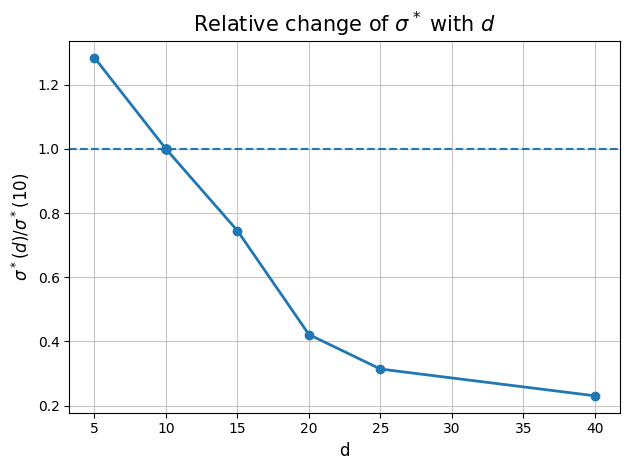
\includegraphics[width=0.6\textwidth]{pic/d40_v2.png}
  \caption{Характер зависимости $\sigma^*$ от размерности $d$}
\end{figure}
\newline
На графике построена зависимость $\frac{\sigma^*(d)}{\sigma^*(10)}$ для наглядности. \newline
Результаты эксперимента показывают, что при увеличении $d$ значение $\sigma^*$ стремительно уменьшается, поэтому в рассматриваемой задаче разумно использовать небольшие значения $d$, порядка $10$, чтобы сэмплирование в данном подпространстве было эффективно. \newline
Перейдём к проверке качества оценки $R_{\psi}$ и 
$\sigma^*$. Для этого рассматривалось гауссовское сэмплирование в подпространстве наибольшей кривизны:
$$\mathbf{w} = \mathbf{w}^{*} + \mathbf{U}_d \mathbf{z}$$ 
$$\mathbf{z} \sim \mathcal{N}(\mathbf{0}, \sigma^2 \mathbf{I}_d)$$
Для $\sigma = \alpha\sigma^*$ при разных $\alpha > 0$. В эксперименте были рассмотрены $\alpha \in [1, 101]$ с шагом $10$.
Для каждой точки вычислялась следующая величина:

$$\Gamma(\mathbf{w}) =  \frac{|\mathcal{L}(\mathbf{w})|}{|\mathcal{L}(\mathbf{w}^*) + \nabla \mathcal{L}(\mathbf{w}^*)^T \mathbf{U}_d \mathbf{z} + \frac{1}{2} \mathbf{z}^T \mathbf{H}_d \mathbf{z}| + \delta}$$

Где малое $\delta > 0$ добавляется для предотвращения деления на 0. \newline
$\Gamma(\mathbf{w})$ отвечает за отношение истинного значения функции потерь в точке $\mathbf{w}$ к её квадратичной аппроксимации Тейлора. \newline
При оптимальном выборе параметра $\sigma^*$ отношение будет близко к 1, а при увеличении $\alpha$ точность аппроксимации будет ухудшаться.
Построим график зависимости $\Gamma(\alpha)$ для медианного значения сэмплирования и для нескольких случайных точек.
На другом графике также построим зависимость $|\Gamma(\alpha) - 1|$ от $\alpha$ для лучшей иллюстрации.

\begin{figure}[h]
    \centering
    \begin{subfigure}[t]{0.49\linewidth}
        \centering
        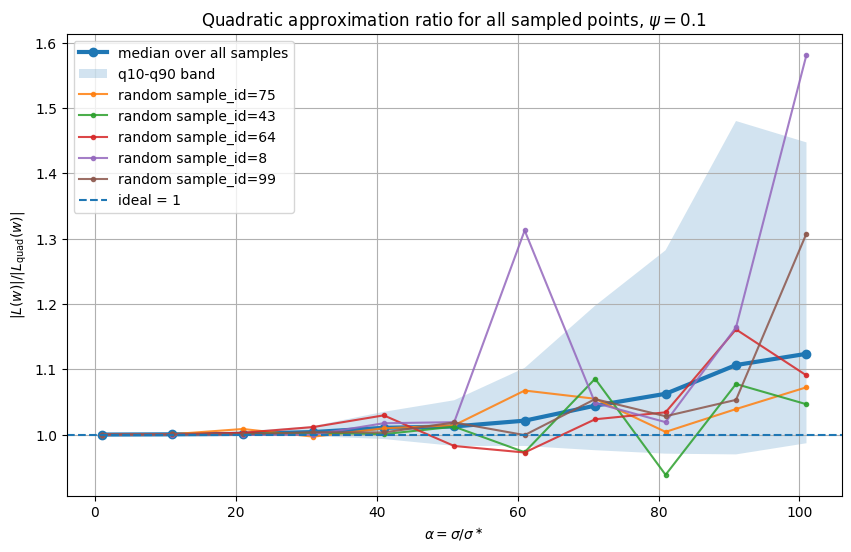
\includegraphics[width=\linewidth]{pic/finally_g-a.png}
        \caption{Зависимость $\Gamma(\alpha)$}
        \label{fig:first}
    \end{subfigure}
    \hfill
    \begin{subfigure}[t]{0.49\linewidth}
        \centering
        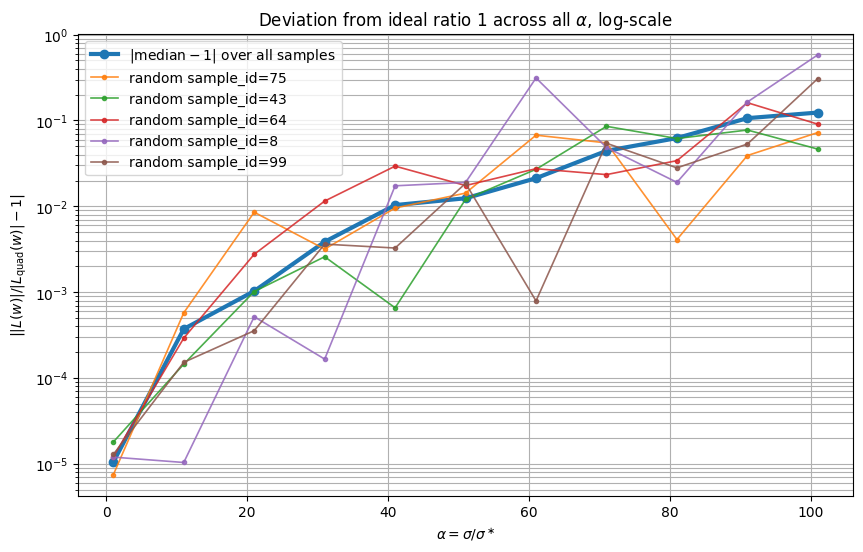
\includegraphics[width=\linewidth]{pic/finally_g-1.png}
        \caption{Зависимость $|\Gamma(\alpha) - 1|$ от $\alpha$, $log$-шкала}
        \label{fig:second}
    \end{subfigure}
    \label{fig:two_plots}
\end{figure}
Первый график показывает поведение $\Gamma(\alpha)$ при увеличении $\alpha$: сэмплирование при выбранном параметре $\sigma^*$ действительно отражает свойства окрестности минимума, в которой корректна аппроксимация Тейлора 2 порядка. Для небольших значений $\alpha$ отношение $\Gamma(\alpha)$ остаётся близким к 1, однако при дальнейшем его увеличении корректность аппроксимации нарушается. \newline
Результаты второго эксперимента показывают точность приближения $\mathcal{L}(\mathbf{w}^*)$ при разных $\alpha$. Видно, что в точке 1, то есть в случае $\sigma = \sigma^*$, квадратичная аппроксимация выполняется с высокой точностью, однако при увеличении $\alpha$ ошибка стремительно растёт.\newline
Вычислительный эксперимент показал, что полученные теоретически значения $R_{\psi}$ и $\sigma^*$ действительно отражают свойства окрестности минимума, в которой аппроксимация Тейлора 2 порядка выполняется с высокой точностью. По графикам видно, что выбор $\sigma^*$ несколько избыточен, однако это объясняется неточностью в вычислении константы Липшица и выбором гиперпараметров $\psi$ и $\varepsilon$. \newline
Следовательно, теоретические результаты подтверждаются вычислительным экспериментом с хорошей точностью.
\section{Выводы}

В работе предложен метод адаптивного выбора параметра гауссовского сэмплирования $\sigma^*$ для исследования оптимизационной поверхности в окрестности минимума и получено выражение для характерного радиуса $R_\psi$ шара с центром в минимуме функции потерь, в котором аппроксимация Тейлора 2 порядка выполняется с заданной точностью. \newline
Проведён вычислительный эксперимент для модели ResNet-18 на датасете CIFAR-10. Он подтверждает корректность полученной оценки: при значениях $\frac{\sigma^*}{\sigma}$ порядка 1 квадратичная аппроксимация хорошо приближает функцию потерь, в то время как при увеличении $\sigma$ точность значительно падает.

Было показано, что величина $\sigma^*$ существенно зависит от размерности подпространства наибольшей кривизны и убывает при росте $d$. Это показывает важность выбора параметра $d$ в будущих исследованиях.

Таким образом, полученные результаты подтверждают практическую применимость предложенного метода выбора параметров. Перспективным направлением дальнейших исследований является проверка корректности критериев Quadratic Monte-Carlo и Gaussian-moment quadratic estimator с учётом полученных выражений для параметров $\sigma$ и $R_\psi$. Ещё одним важным направлением является построения графика $\sigma(d)$ для больших $d$ для лучшего понимания зависимости и выбора $d$ в будущих исследованиях.

\bibliographystyle{unsrt}
\bibliography{xd}

\end{document}  
